\documentclass[a4paper, 11pt]{article}
\usepackage[english]{babel}
\usepackage{fullpage}

\usepackage[pdftex]{graphicx}
\graphicspath{{../pdf/}{../jpeg/}}
\DeclareGraphicsExtensions{.pdf,.jpeg,.png}

% ----------------------------------------------

% Definitions of languages: --------------------
\usepackage{listings}
\lstdefinestyle{cStyle}{
  basicstyle=\scriptsize,
  breakatwhitespace=false,
  breaklines=true,
  captionpos=b,
  keepspaces=true,
  numbersep=5pt,
  showspaces=false,
  gobble=4,
  tabsize=4,
  showstringspaces=false,
  showtabs=false,
}
\renewcommand*{\lstlistingname}{Code}

% ----------------------------------------------

\renewcommand*{\i}{\textit}

\begin{document}

\noindent
\large\textbf{CES-25 Computer Networks and Internet} \\
\textbf{2th Activity} \\
\normalsize Prof Lourenço  \\
Carlos Matheus Barros da Silva \hfill September 2019

\section{Implementation}

All the code was implemented using Python 3. The complite code can be seen on the Repository\footnote{https://github.com/CarlosMatheus/ftp-server}.

The code was divided into five files, beeing four of them classes. The classes are \i{Commander}, \i{Client}, \i{Server}, \i{FileManager} and there are a utility file called \i{utils}.

\subsection{Commander}

It is an abstract class that will define methods related to command line. The classes \i{Server} and \i{Client} will inherit from \i{Commander}.

The commands methods parsing and routing are provided by the \i{Commander} abstract class they will be routed to the corresopnding abstract method that are implemented by the \i{Server} and the \i{Client} classes.

Therefore if \i{Commander} receive ``cd ./..'' it will first split the message by spaces and then pass the first element to a command hash that will lead to the specific method or to the \i{unknown} method in case no method related to that name exists, the others elemenst of the splited string are passed as arguments for the method and each function will deal independenlty with it.

\subsection{FileManager}

The \i{FileManager} class is a class that deals with the computer files. Every thing related to read or write files or directories will be done throgh the intermediate \i{FileManager} classe.

Therefore the code will be more specialized and will be better to organize and prevend race conditions on the server when more then one thread are tring to access the shared resources. On that way locks are implemented so that it is garanteed that at most only one thread area accessing the \i{FileManager} methods at the same time.

\i{FileManager} also include path validation and simplification methods, wherefore it can vefiry that ``a/../a/./../a'' is equals to ``a/'', it also verify the vality of a given directory or file. It furthermore checks if the directory that is been accessed is inside the root folder defined by the server, that way it prevets the user to navigate and access every file on the server machine, it just allow the navigation through the files inside root folder defined by server.

\subsection{Server}

It is the class that controls the server, and in order to initiate a server it is just necessary to create a instance of \i{Server}. The server will initialy define the port it will initiate the server and then define a password for the server. The password will be stored as an \i{Sha256} hash of the password given.

When the serve is initialized it will be listening and waiting for new connections, when it receive a new connection request from a client it will inictiate a new server object on a new thread specially for that connection so the main thread will continue waiting new connections, and every connectino already stableshed will have it own thread.

On the specific thread conection, the server will be first waiting for the user provide a message with the correct password hash. Once the user is authenticated the server will be waiting for commands.

The commands methods parsing and routing are provided by the \i{Commander} abstract class they will be routed to the corresopnding abstract method that are implemented by the \i{Server} and the \i{Client} classes.

Therefore if \i{Commander} receive ``cd ./..'' it will first split the message by spaces and then pass the first element to a command hash that will lead to the specific method or to the \i{unknown} method in case no method related to that name exists, the others elemenst of the splited string are passed as arguments for the method and each function will deal independenlty with it.

So for the commands that the server will be able to receive, all the commands requested were implemented fallowing the arguments utilization. Thus the \i{cd}, \i{ls}, \i{pwd}, \i{mkdir}, \i{rmdir}, \i{get}, \i{put}, \i{delete}, \i{close}, \i{open} and \i{quit} were implemented.

Their complete utilization fallows stricly the suggestion on the Activity proposal. Besides for the \i{get} and \i{put} it can be used with one more optional argument definig the folder to interact.

\subsection{Client}

This class implements the client side application. In order to run the client side application just need to create an instance of this class.

When initate the client application it will be prompt a command line. At first until the user are not connected and authenticated to a server all commands are blocked except \i{open} and \i{quit}. When the client calls open passing the arguments to the server address and port it will be asked the server password. So for example ``open 0.0.0.0:8080'' will try connect to the server on the \i{0.0.0.0} addess at \i{8080} port.

After connect the server will ask the password, once the user prompts the password the value will be hashed using \i{Sha256} and sent to the server and the server will answer telling if it is authenticated.

Once authenticated, the client will be waiting for the user input the command to send it to the server. Every command the user type will be parsed through the \i{Commander} methods and routed to the respective method, on it will fallow the respective logic locally before send the message to the server with the command and arguments. If there are any error detectable from the client side it will the shown the errors message on the client side before send to the server.

\section*{Implementation}

\subsection*{Suggested Test Case}

As It was suggested, it was conducted a test with 3 terminal windows, on each one was opened one task of the program as shown in the Code \ref{code_code1}.

The test was made according to the model represented on Figure \ref{img_task1}. The results can be seen on the terminal windows shown from Figure \ref{img_task1_example_window1} to Figure \ref{img_task1_example_window3}.

% \begin{figure}[h]
%   \begin{center}
%   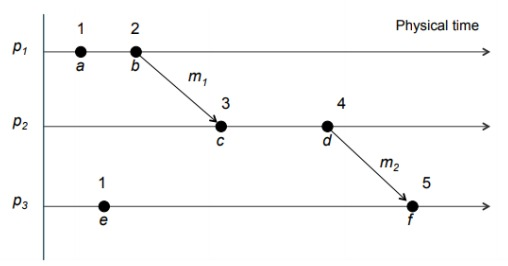
\includegraphics[width=4in]{./imgs/task1_example_model.jpeg}
%   \caption{Model representing the execution of Task 1 example test case.}
%   \label{img_task1}
%   \end{center}
% \end{figure}
%
% \lstinputlisting[
%     language=python,
%     caption={Code that was run on each of the 3 terminal window on the execution of Task 1 example test case.},
%     label={code_code1},
%     style=cStyle,
% ]{./code1.txt}
%
% \begin{figure}[h]
%   \begin{center}
%   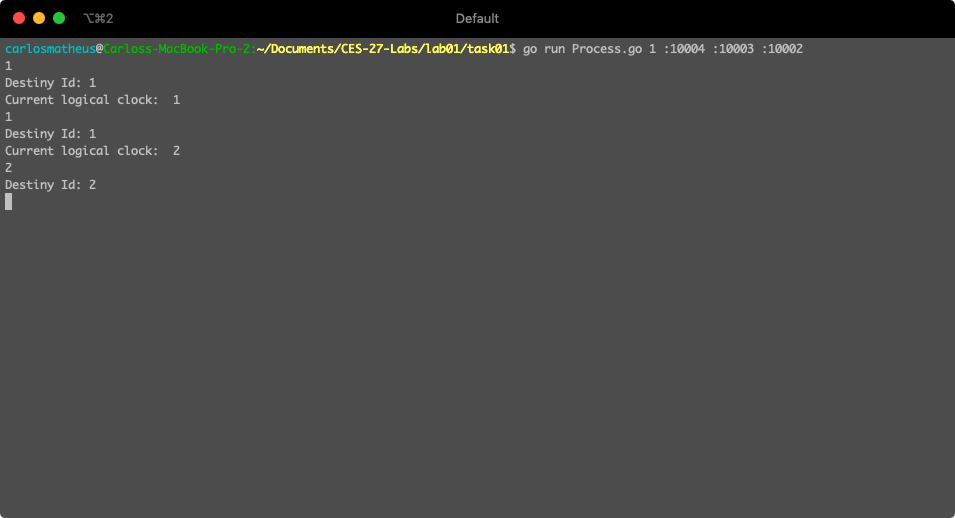
\includegraphics[width=4.5in]{./imgs/task1_example_window1.png}
%   \caption{Window 1 after execution of Task 1 example test case.}
%   \label{img_task1_example_window1}
%   \end{center}
% \end{figure}
%
% \begin{figure}[h]
%   \begin{center}
%   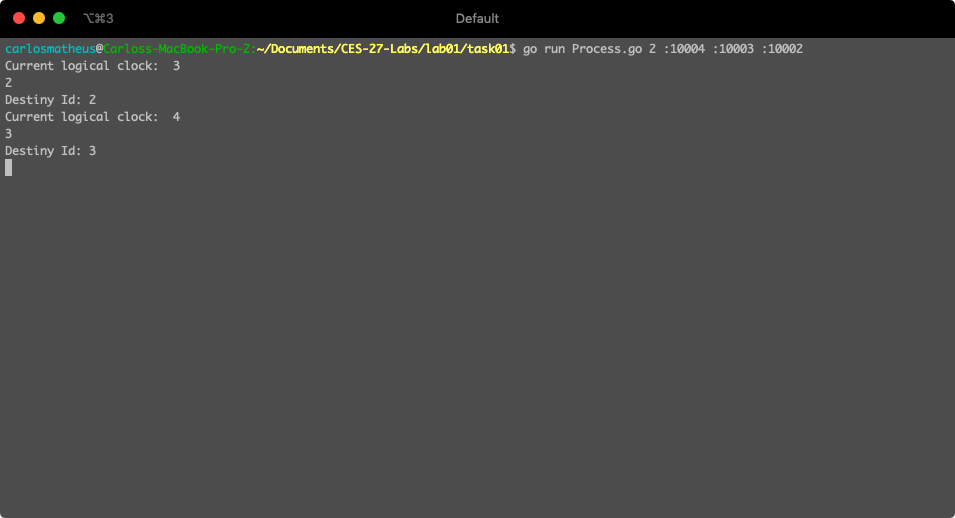
\includegraphics[width=4.5in]{./imgs/task1_example_window2.png}
%   \caption{Window 2 after execution of Task 1 example test case.}
%   \label{img_task1_example_window2}
%   \end{center}
% \end{figure}
%
% \begin{figure}[h]
%   \begin{center}
%   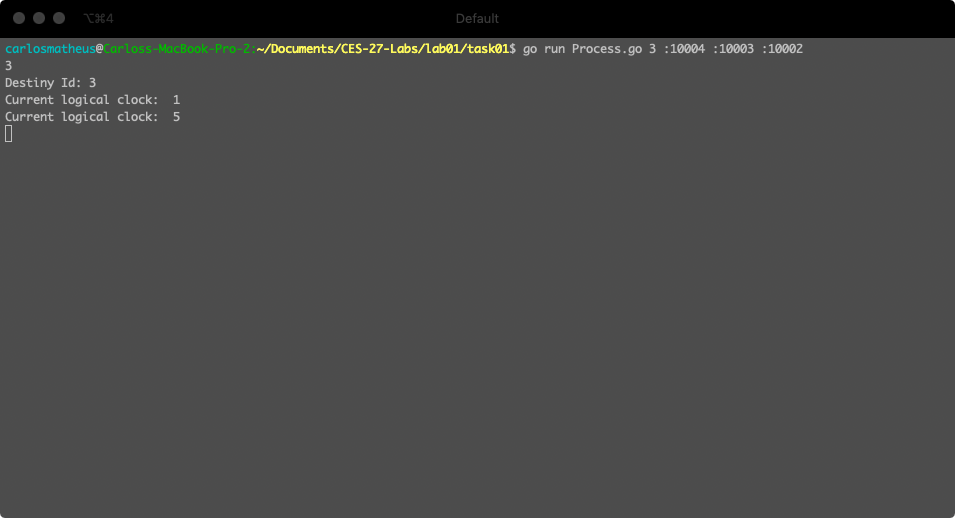
\includegraphics[width=4.5in]{./imgs/task1_example_window3.png}
%   \caption{Window 3 after execution of Task 1 example test case.}
%   \label{img_task1_example_window3}
%   \end{center}
% \end{figure}

As expected, the logical clock on each process was updated to the bigger one, if the incomming message logical clock time was greater than the actual time on that process, and then it was also increased by one. This logic was applied and because of it the simulation on the terminals matched the model represented on Figure \ref{img_task1}.

\subsection*{Built Test Case}

It was built a test case with 4 terminal windows, on each one was opened one task of the program as shown in the Code \ref{code_img_task1_built_case}.

The test was made according to the model represented on Figure \ref{img_task1}. The results can be seen on the terminal windows shown from Figure \ref{img_task1_built_case_window1} to Figure \ref{img_task1_built_case_window4}.


\begin{figure}[h]
  \begin{center}
  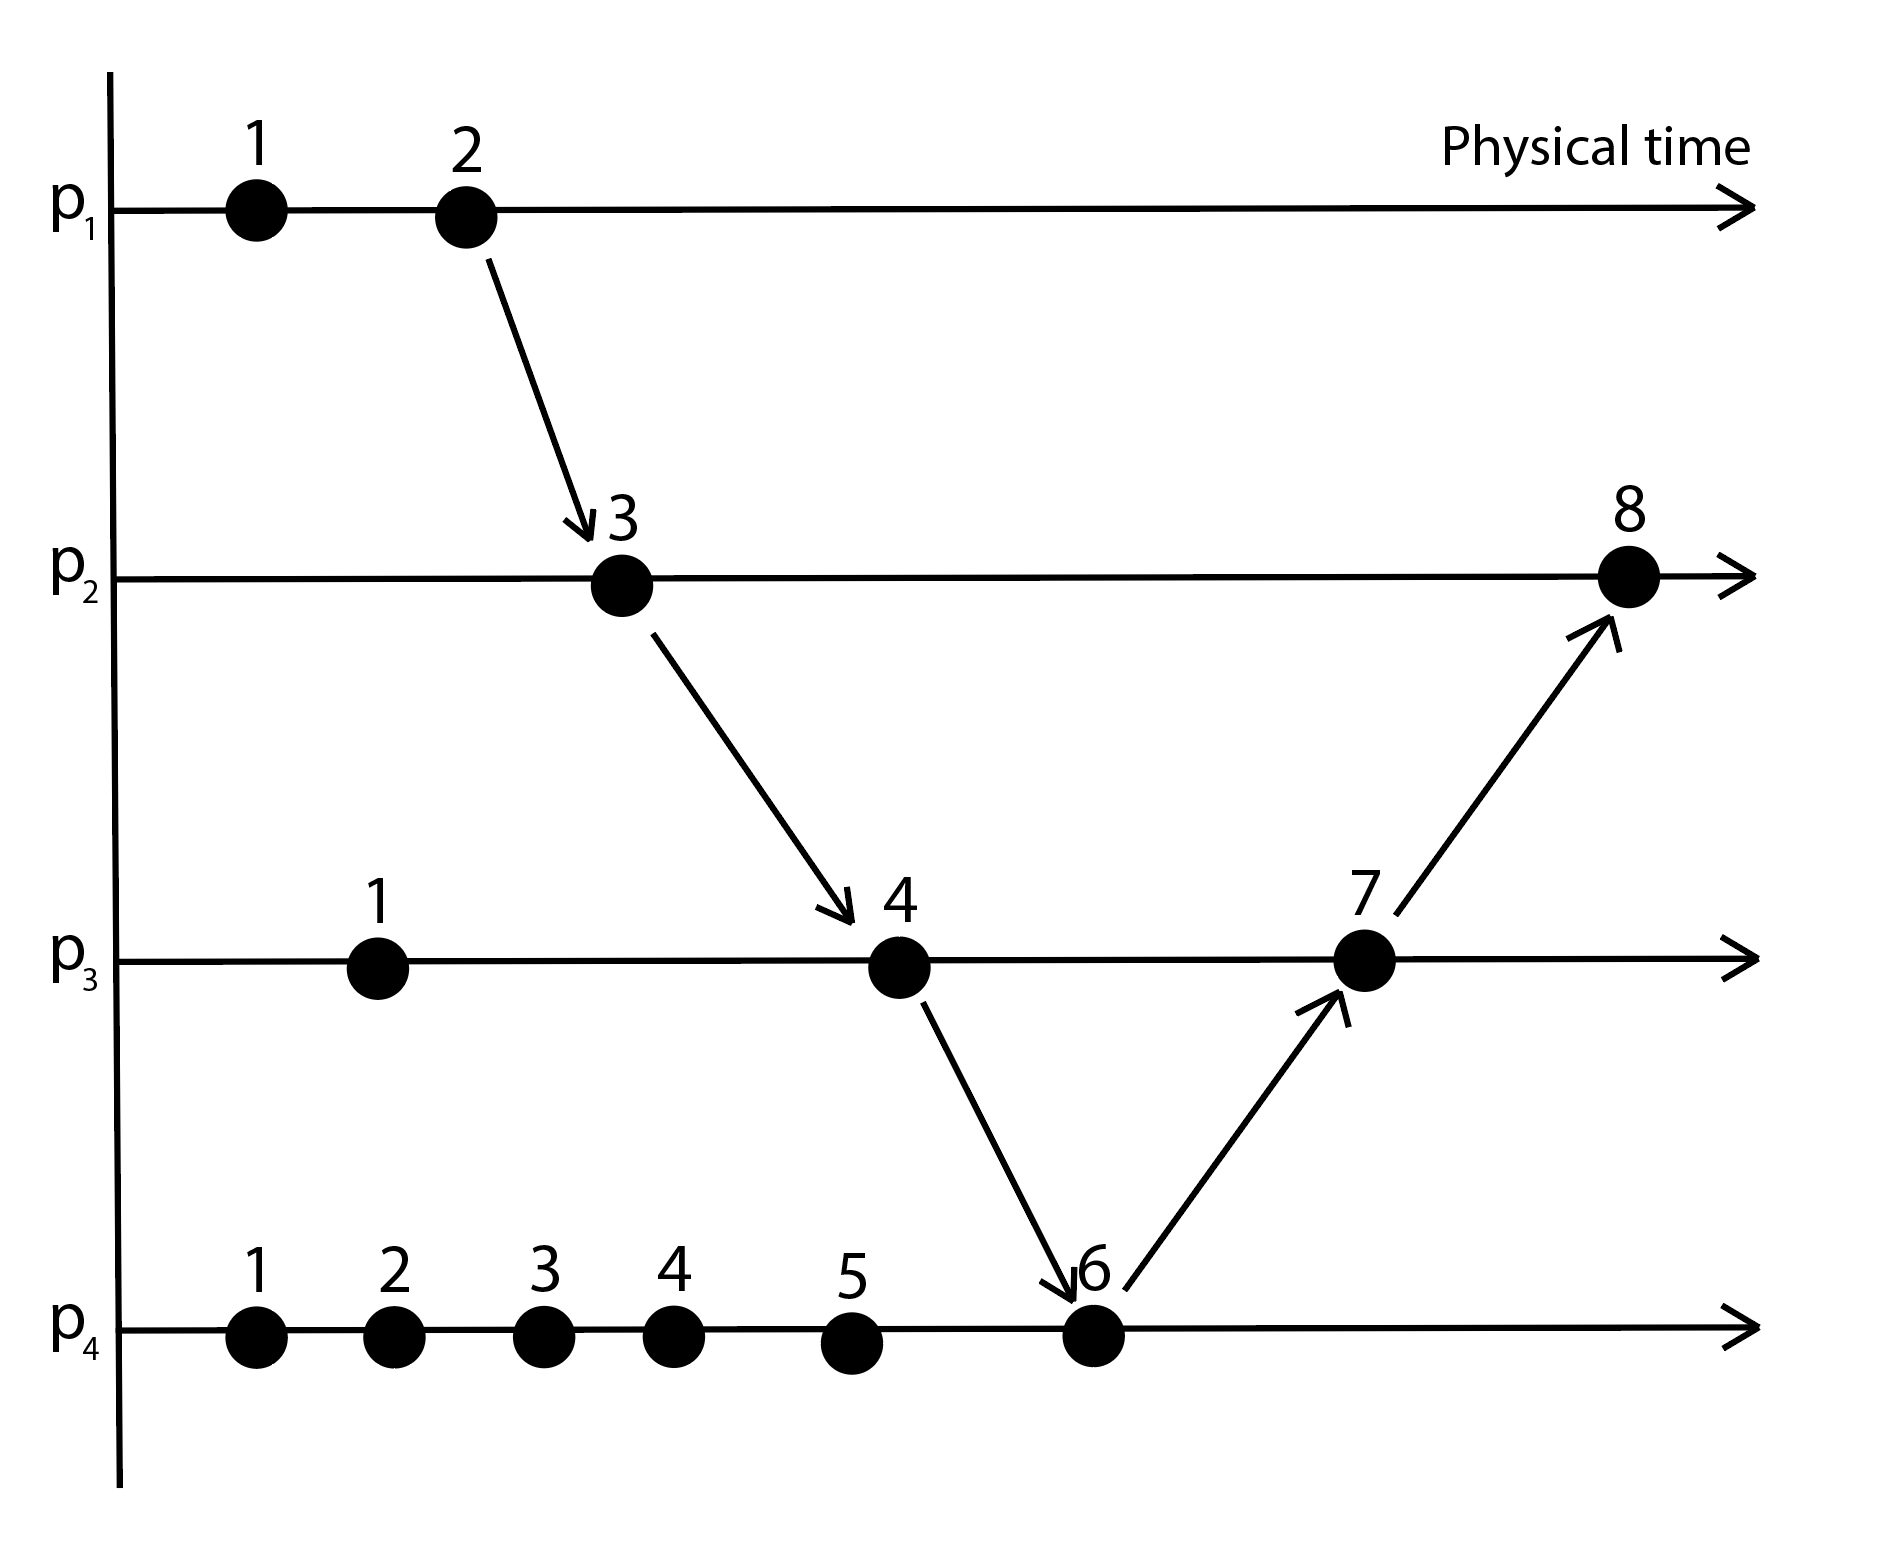
\includegraphics[width=3in]{./imgs/task1_built_case_model.png}
  \caption{Model representing the execution of Task 1 built test case.}
  \label{img_task1_built_case_model}
  \end{center}
\end{figure}



\lstinputlisting[
    language=python,
    caption={Code that was run on each of the 4 terminal window on the execution of Task 1 built test case.},
    label={code_img_task1_built_case},
    style=cStyle,
]{./code2.txt}


\begin{figure}[h]
  \begin{center}
  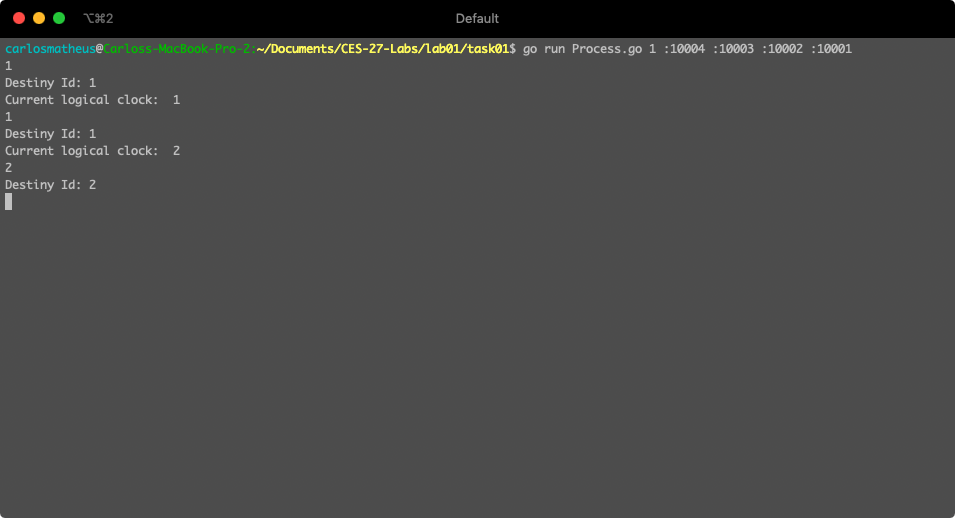
\includegraphics[width=4.5in]{./imgs/task1_buit_test_window1.png}
  \caption{Window 1 after execution of Task 1 built test case.}
  \label{img_task1_built_case_window1}
  \end{center}
\end{figure}

\begin{figure}[h]
  \begin{center}
  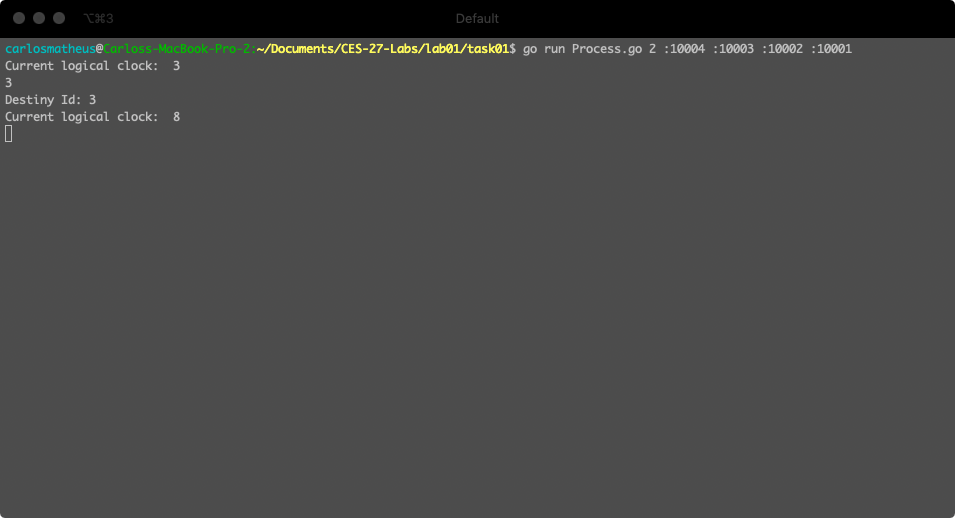
\includegraphics[width=4.5in]{./imgs/task1_buit_test_window2.png}
  \caption{Window 2 after execution of Task 1 built test case.}
  \label{img_task1_built_case_window2}
  \end{center}
\end{figure}

\begin{figure}[h]
  \begin{center}
  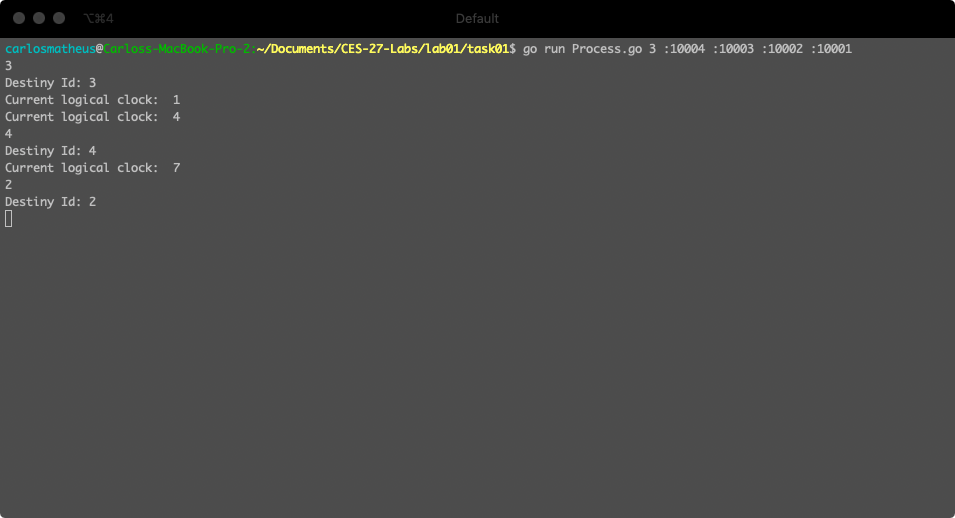
\includegraphics[width=4.5in]{./imgs/task1_buit_test_window3.png}
  \caption{Window 3 after execution of Task 1 built test case.}
  \label{img_task1_built_case_window3}
  \end{center}
\end{figure}

\begin{figure}[h]
  \begin{center}
  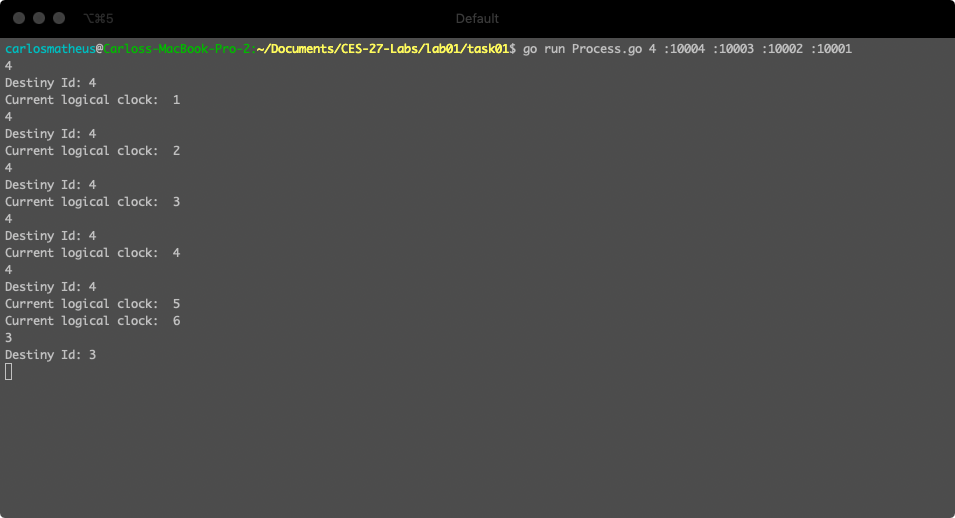
\includegraphics[width=4.5in]{./imgs/task1_buit_test_window4.png}
  \caption{Window 4 after execution of Task 1 built test case.}
  \label{img_task1_built_case_window4}
  \end{center}
\end{figure}

As expected, the logical clock on each process was updated to the bigger one, if the incomming message logical clock time was greater than the actual time on that process, and then it was also increased by one. This logic was applied and because of it the simulation on the terminals matched the model represented on Figure \ref{img_task1}.

\section*{Task 2}

\subsection*{Suggested Test Case}

As It was suggested, it was conducted a test with 3 terminal windows, on each one was opened one task of the program as shown in the Code \ref{task2_code_code1}.

The test was made according to the model represented on Figure \ref{task2_example_model}. The results can be seen on the terminal windows shown from Figure \ref{img_task2_example_window1} to Figure \ref{img_task2_example_window3}.

\begin{figure}[h]
  \begin{center}
  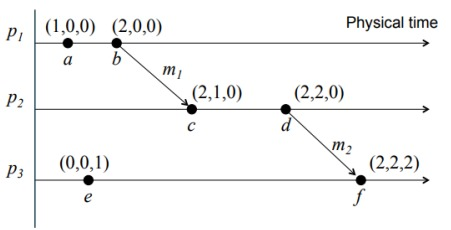
\includegraphics[width=4in]{./imgs/task2_example_model.jpeg}
  \caption{Model representing the execution of Task 1 example test case.}
  \label{task2_example_model}
  \end{center}
\end{figure}

\lstinputlisting[
    language=python,
    caption={Code that was run on each of the 3 terminal window on the execution of Task 2 example test case.},
    label={task2_code_code1},
    style=cStyle,
]{./code1.txt}

\begin{figure}[h]
  \begin{center}
  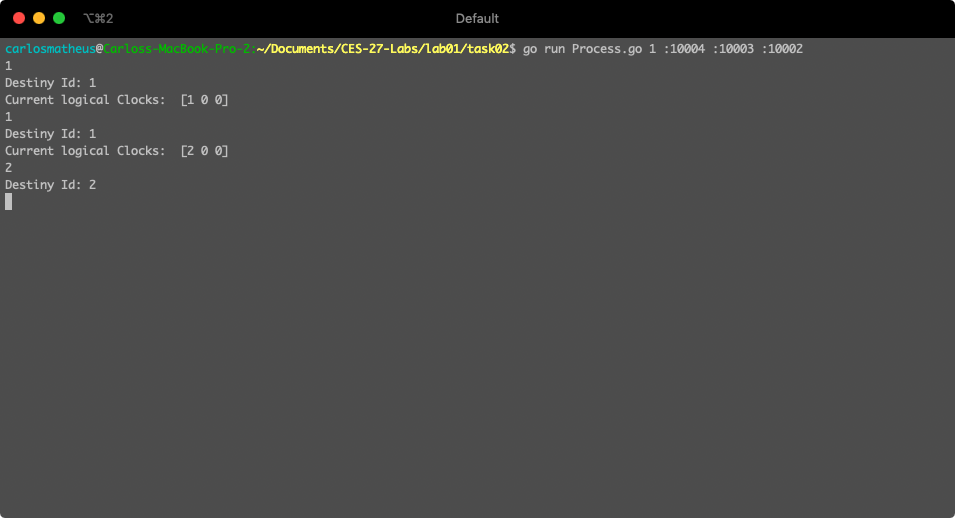
\includegraphics[width=4.5in]{./imgs/task2_example_window1.png}
  \caption{Window 1 after execution of Task 2 example test case.}
  \label{img_task2_example_window1}
  \end{center}
\end{figure}

\begin{figure}[h]
  \begin{center}
  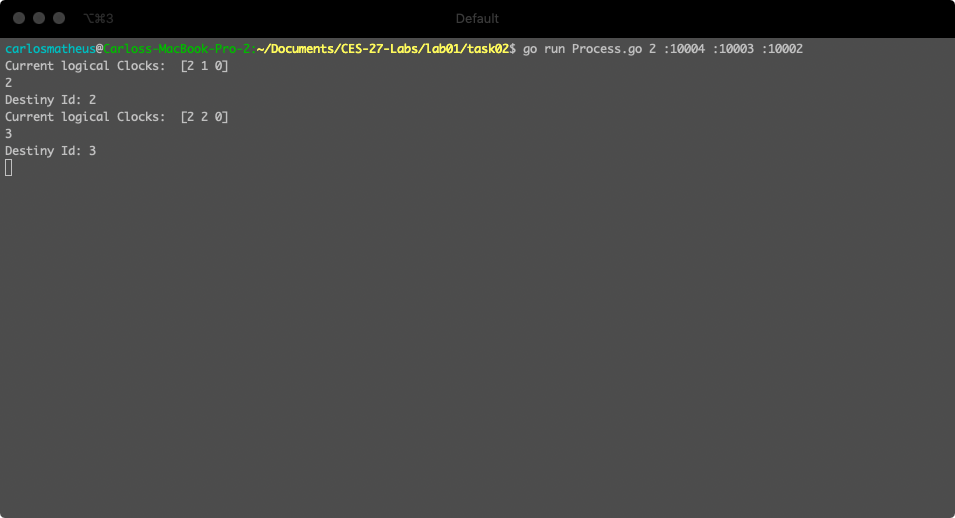
\includegraphics[width=4.5in]{./imgs/task2_example_window2.png}
  \caption{Window 2 after execution of Task 2 example test case.}
  \label{img_task2_example_window2}
  \end{center}
\end{figure}

\begin{figure}[h]
  \begin{center}
  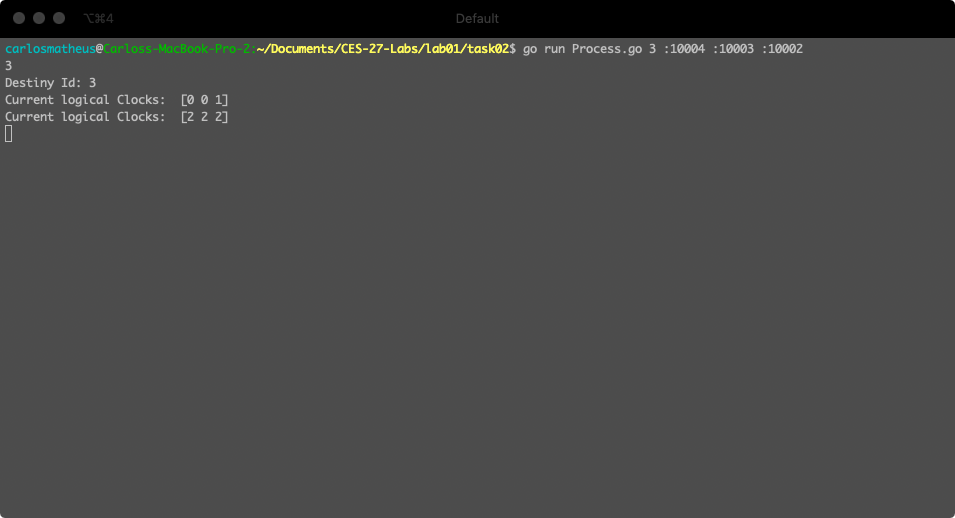
\includegraphics[width=4.5in]{./imgs/task2_example_window3.png}
  \caption{Window 3 after execution of Task 2 example test case.}
  \label{img_task2_example_window3}
  \end{center}
\end{figure}

% need to change this part ==========
As expected, the logical clock on each process was updated to the bigger one, if the incomming message logical clock time was greater than the actual time on that process, and then it was also increased by one. This logic was applied and because of it the simulation on the terminals matched the model represented on Figure \ref{task2_example_model}.
% ==============================

\subsection*{Built Test Case}

It was built a test case with 3 terminal windows, on each one was opened one task of the program as shown in the Code \ref{code_img_task2_built_case}.

The test was made according to the model represented on Figure \ref{img_task2_built_case_model}. The results can be seen on the terminal windows shown from Figure \ref{img_task2_built_case_window1} to Figure \ref{img_task2_built_case_window3}.

\begin{figure}[h]
  \begin{center}
  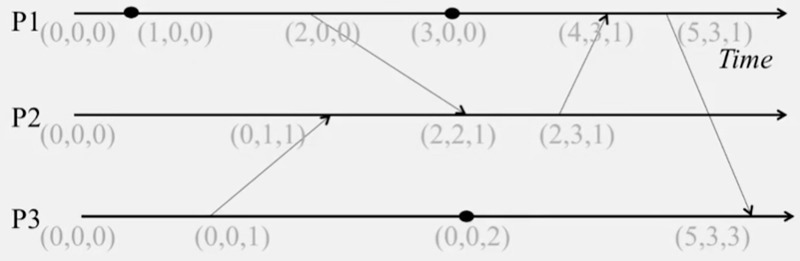
\includegraphics[width=4in]{./imgs/task2_built_case_model.jpeg}
  \caption{Model representing the execution of Task 2 built test case.}
  \label{img_task2_built_case_model}
  \end{center}
\end{figure}

\lstinputlisting[
    language=python,
    caption={Code that was run on each of the 3 terminal window on the execution of Task 2 built test case.},
    label={code_img_task2_built_case},
    style=cStyle,
]{./code2.txt}

\begin{figure}[h]
  \begin{center}
  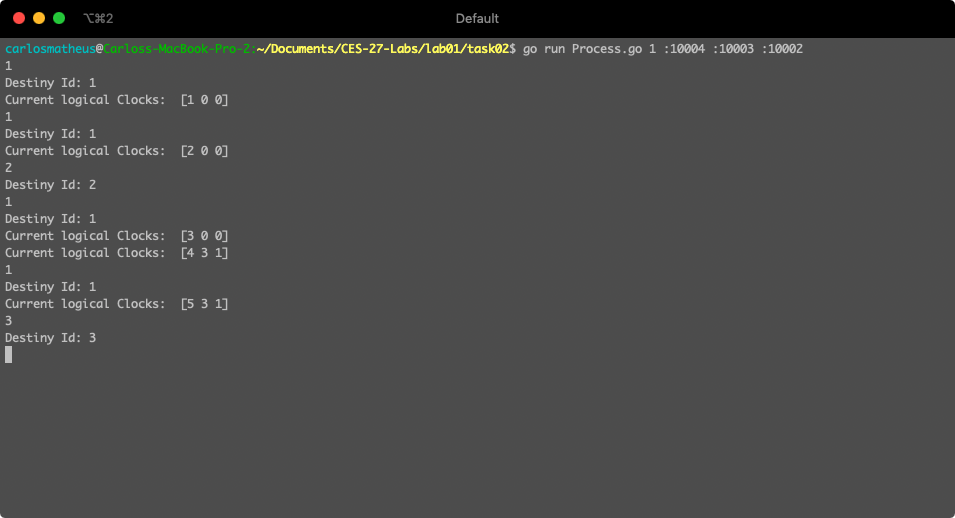
\includegraphics[width=4.5in]{./imgs/task2_buit_test_window1.png}
  \caption{Window 1 after execution of Task 2 built test case.}
  \label{img_task2_built_case_window1}
  \end{center}
\end{figure}

\begin{figure}[h]
  \begin{center}
  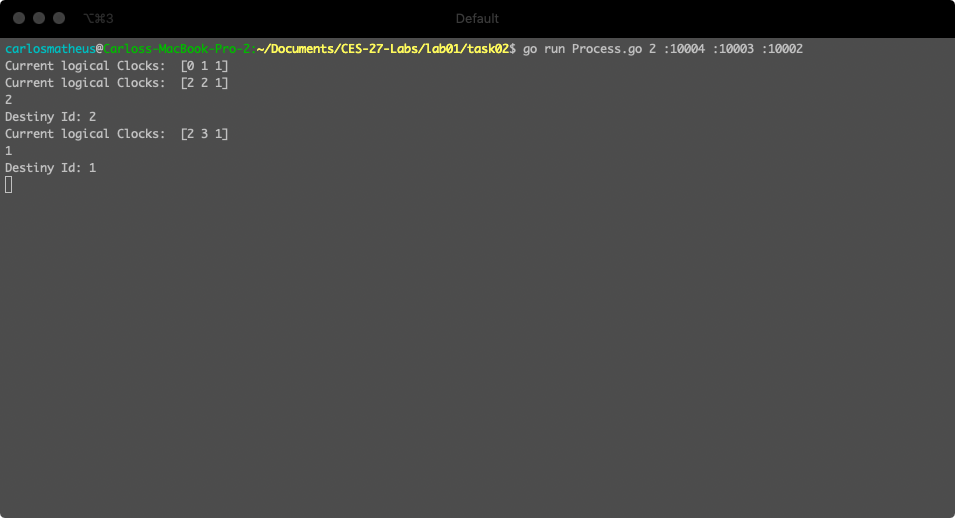
\includegraphics[width=4.5in]{./imgs/task2_buit_test_window2.png}
  \caption{Window 2 after execution of Task 2 built test case.}
  \label{img_task2_built_case_window2}
  \end{center}
\end{figure}

\begin{figure}[h]
  \begin{center}
  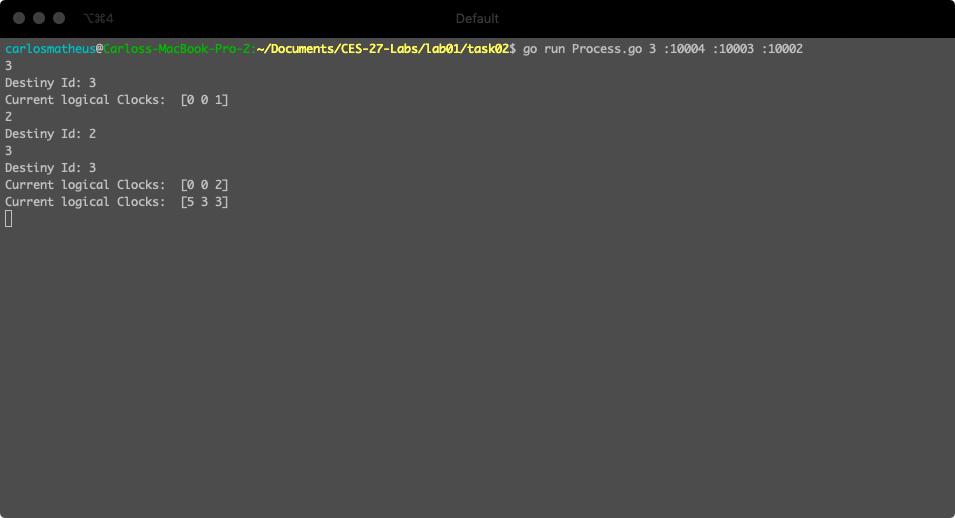
\includegraphics[width=4.5in]{./imgs/task2_buit_test_window3.png}
  \caption{Window 3 after execution of Task 2 built test case.}
  \label{img_task2_built_case_window3}
  \end{center}
\end{figure}

As expected, the logical clock on each process was updated to the bigger one, if the incomming message logical clock time was greater than the actual time on that process, and then it was also increased by one. This logic was applied and because of it the simulation on the terminals matched the model represented on Figure \ref{img_task2_built_case_model}.

% \newpage
% \bibliographystyle{plain}
% \bibliography{bibliography.bib}

\end{document}
